\clearpage
\textcolor{blue}{EQ: Our main analysis here is using the quarterly sample and login days. We are using random 30\% of the data, 27,021 accounts. In Appendix, we have the results for (1) replications using sub-samples of equal bin size (quarterly sample ),  (2) replications for monthly and annual samples (login days), (3) replication of the main analysis with sell days (quarterly sample), (4) random sells (using the quarterly sample). We also have analysis with (5) all data showing no patterns.   }

\begin{figure}[hbt!]
	\caption{Leftmost Stock Price Digit and Probability of Sale, Quarterly Sample}%
	\label{fig:left_digit_sell}%
	\centering%	
	\bigskip
	\subfigure[Price Increasing]{
		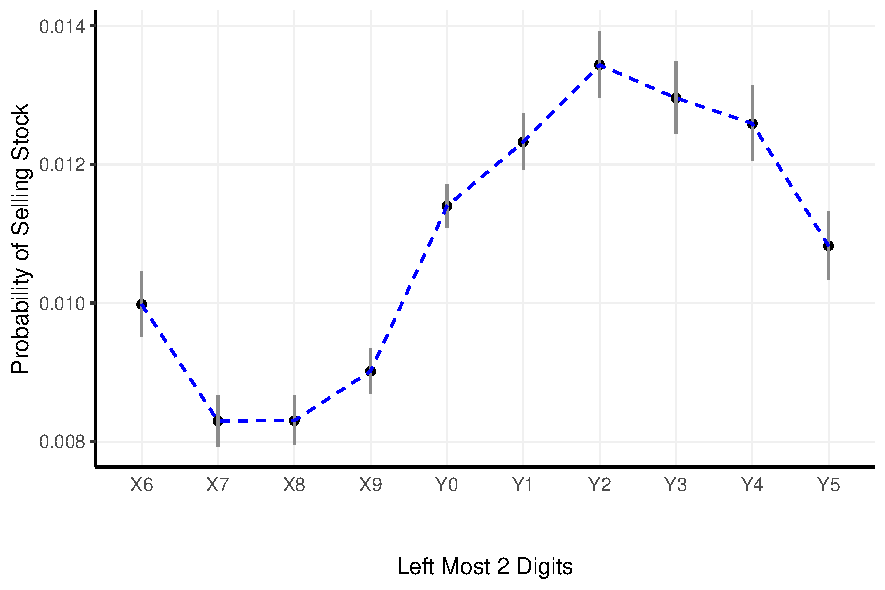
\includegraphics[width=0.45\textwidth]{figures/Left2increase_probCI_quarter.pdf}
		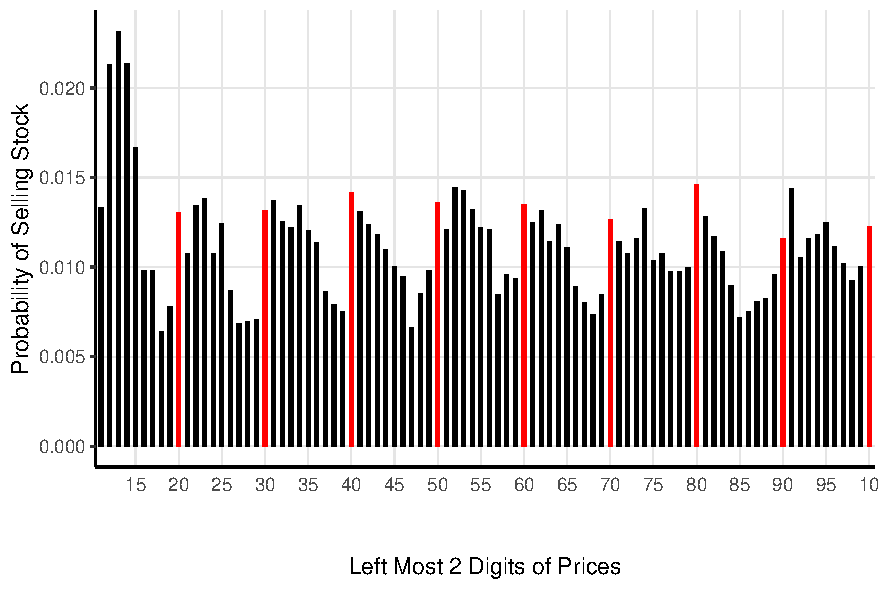
\includegraphics[width=0.45\textwidth]{figures/2left_increase_quarter.pdf}	
	}
	\subfigure[Price Decreasing]{
		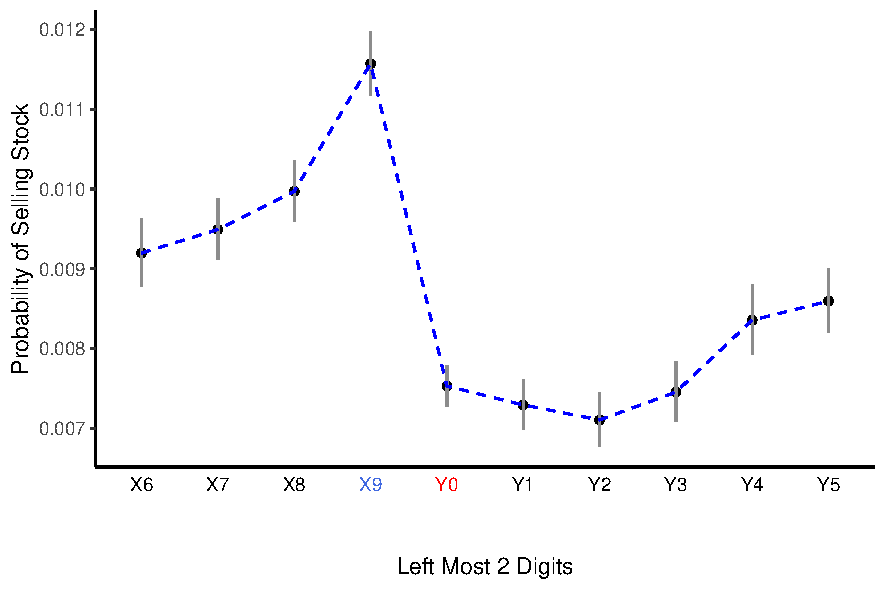
\includegraphics[width=0.45\textwidth]{figures/Left2decrease_probCI_quarter.pdf}
		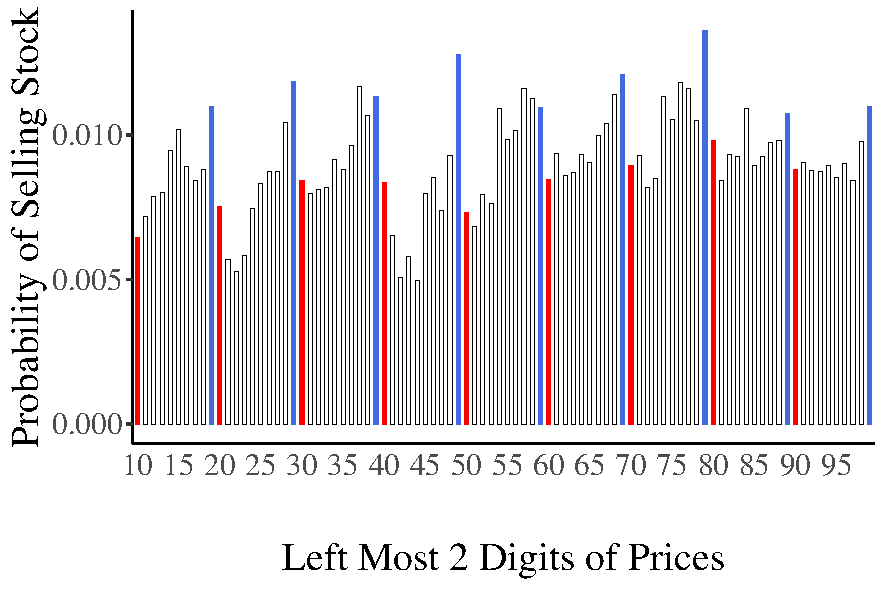
\includegraphics[width=0.45\textwidth]{figures/2left_decrease_quarter.pdf}	
	}
	\fignote{£$Y$ in the X-axes is equivalent to £$X+1$ (e.g., £X9 could include £0.19, £1.9, £19, etc., while £Y0 could include £0.20, £2.0, £20, etc.).}
\end{figure}


